%% main.tex
%% Main Document for ITS Thesis Template
%% Based on Panduan Penyusunan Tesis Program Magister ITS 2021
%%
%% COMPILATION INSTRUCTIONS:
%% 1. Compile cover.tex first:
%%    pdflatex cover.tex
%%
%% 2. Then compile main.tex:
%%    pdflatex main.tex
%%    bibtex main
%%    pdflatex main.tex
%%    pdflatex main.tex

\documentclass{its-thesis}

%% ============================================================================
%% THESIS INFORMATION - ISI DATA TESIS ANDA DI SINI
%% ============================================================================

% Kode Tesis (sesuai mata kuliah)
\thesisCode{EF235401}

% Judul Tesis (Indonesia) - Capitalize Each Word sesuai EYD
% Maksimum 20 kata
\titleID{Judul Tesis Ditulis dengan Capitalize Each Word Sesuai EYD}

% Thesis Title (English)
\titleEN{Thesis Title Written in English with Proper Capitalization}

% Informasi Penulis
\authorname{NAMA MAHASISWA}
\studentid{NRP MAHASISWA}

% Informasi Dosen Pembimbing
\supervisorOne{Prof. Dr. Nama Pembimbing 1, S.T., M.T.}
\supervisorOneNIP{19XXXXXX XXXXXX X XXX}
\supervisorTwo{Dr. Nama Pembimbing 2, S.Kom., M.Kom.}
\supervisorTwoNIP{19XXXXXX XXXXXX X XXX}

% Informasi Penguji
\examinerOne{Dr. Nama Penguji 1, S.T., M.T.}
\examinerOneNIP{19XXXXXX XXXXXX X XXX}
\examinerTwo{Dr. Nama Penguji 2, S.Kom., M.Kom.}
\examinerTwoNIP{19XXXXXX XXXXXX X XXX}

% Informasi Ujian dan Wisuda
\examDate{DD Bulan YYYY}
\graduationPeriod{Semester Genap/Ganjil YYYY/YYYY}

% Informasi Program Studi
\studyProgram{S2 Teknik Informatika}
\expertise{Manajemen Cerdas Informasi}
\department{Teknik Informatika}
\faculty{Teknologi Elektro dan Informatika Cerdas}

% Tahun Tesis
\thesisYear{2025}

% Gelar yang diperoleh
% \degree{Magister Teknik (M.T.)}

% Kepala Departemen
\deptHead{Prof. Dr. Nama Kaprodi, S.T., M.T.}
\deptHeadNIP{19XXXXXX XXXXXX X XXX}

% Kata Kunci (3-5 kata kunci, diurutkan alfabetis)
\keywordsID{Kata Kunci 1, Kata Kunci 2, Kata Kunci 3, Kata Kunci 4, Kata Kunci 5}
\keywordsEN{Keyword 1, Keyword 2, Keyword 3, Keyword 4, Keyword 5}

%% ============================================================================
%% BIBLIOGRAPHY FILE
%% ============================================================================

\addbibresource{references.bib}

%% ============================================================================
%% DOCUMENT BEGINS
%% ============================================================================

\begin{document}

%% Override babel names explicitly (ensure they're set)
\renewcommand{\contentsname}{DAFTAR ISI}
\renewcommand{\listfigurename}{DAFTAR GAMBAR}
\renewcommand{\listtablename}{DAFTAR TABEL}
\renewcommand{\chaptername}{BAB}
\renewcommand{\bibname}{DAFTAR PUSTAKA}

%% ============================================================================
%% COVER PAGE (SAMPUL LUAR) - TANPA NOMOR HALAMAN
%% Compile cover.tex separately first to generate cover.pdf
%% ============================================================================

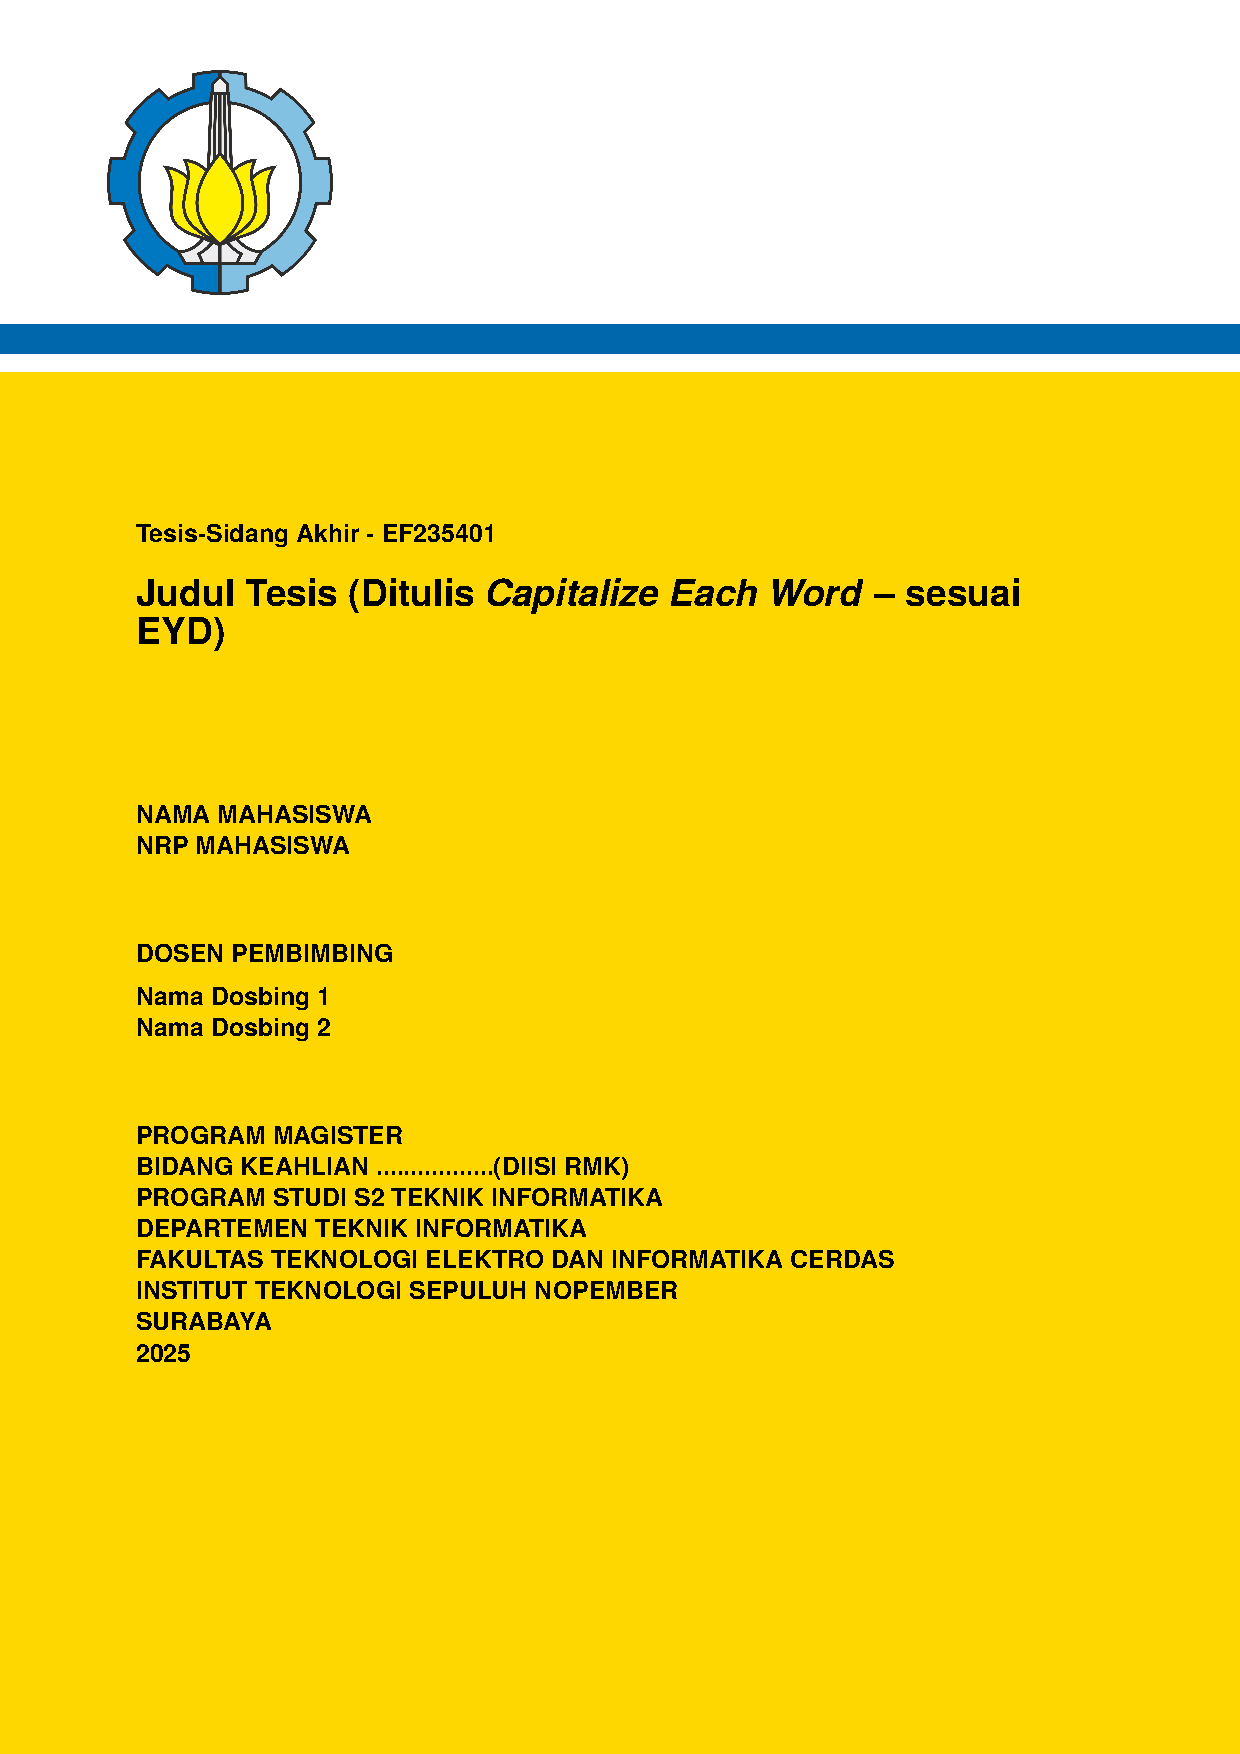
\includepdf[pages=1,pagecommand={\thispagestyle{empty}}]{cover.pdf}

%% ============================================================================
%% FRONT MATTER (BAGIAN AWAL)
%% Penomoran halaman: angka Romawi kecil (i, ii, iii, ...)
%% Halaman Judul dimulai dari halaman i
%% ============================================================================

\pagenumbering{roman}
\setcounter{page}{1}
\pagestyle{plain}

%% ----------------------------------------------------------------------------
%% Halaman Judul (Sampul Dalam) - halaman i
%% File: frontmatter/halaman-judul.tex
%% ----------------------------------------------------------------------------
\newpage
\thispagestyle{plain}
%% halaman-judul.tex
%% Halaman Judul (Sampul Dalam)
%% Format sama dengan cover.tex tapi tanpa background kuning
%% Font: Sans-serif (TeX Gyre Heros) seperti cover
%%
%% EDIT LANGSUNG TEKS DI BAWAH INI SESUAI DATA TESIS ANDA
\newpage
\thispagestyle{plain}
% Temporarily switch to sans-serif font for this page
{
\sffamily % Switch to sans-serif font

% All layout using TikZ for precise positioning
\begin{tikzpicture}[remember picture,overlay]
    % ITS Logo - positioned at top left corner
    \node[anchor=north west] at ([xshift=1.5cm,yshift=-2cm]current page.north west) 
        {
\includegraphics[width=3.5cm]{figures/logo-its.png}};
    
    % Blue stripe - full width
    \fill[ITSBlue] ([yshift=-6cm]current page.north west) rectangle ([yshift=-6.5cm]current page.north east);
    
    % Content - positioned below blue stripe
    % UBAH NILAI yshift=-8cm UNTUK MENGATUR JARAK DARI ATAS
    \node[anchor=north west, text width=15cm] at ([xshift=2.0cm,yshift=-8cm]current page.north west) {
        \begin{minipage}{15cm}
        \begin{onehalfspace}
        
        %% ===== KODE TESIS =====
        {\fontsize{12pt}{14pt}\selectfont\bfseries Tesis-Sidang Akhir - EF235401}
        
        \vspace{0.4cm}
        
        %% ===== JUDUL TESIS (18pt bold) =====
        %% Edit judul di sini
        {\fontsize{18pt}{22pt}\selectfont\bfseries 
        Judul Tesis (Ditulis \textit{Capitalize Each Word} – sesuai EYD)}
        
        \vspace{1.8cm}
        
        %% ===== NAMA DAN NRP MAHASISWA =====
        {\fontsize{12pt}{14pt}\selectfont\bfseries 
        NAMA MAHASISWA\\
        NRP MAHASISWA}
        
        \vspace{1cm}
        
        %% ===== DOSEN PEMBIMBING =====
        {\fontsize{12pt}{14pt}\selectfont\bfseries DOSEN PEMBIMBING}
        
        \vspace{0.15cm}
        
        {\fontsize{12pt}{14pt}\selectfont\bfseries 
        Nama Dosbing 1\\
        Nama Dosbing 2}
        
        \vspace{1cm}
        
        %% ===== INFORMASI PROGRAM =====
        {\fontsize{12pt}{14pt}\selectfont\bfseries 
        PROGRAM MAGISTER\\
        BIDANG KEAHLIAN .................(DIISI RMK)\\
        PROGRAM STUDI S2 TEKNIK INFORMATIKA\\
        DEPARTEMEN TEKNIK INFORMATIKA\\
        FAKULTAS TEKNOLOGI ELEKTRO DAN INFORMATIKA CERDAS\\
        INSTITUT TEKNOLOGI SEPULUH NOPEMBER\\
        SURABAYA\\
        TAHUN}
        
        \end{onehalfspace}
        \end{minipage}
    };
\end{tikzpicture}

} % End of sffamily
\phantomsection
\addcontentsline{toc}{chapter}{HALAMAN JUDUL}

%% Halaman Kosong setelah Halaman Judul
\newpage
\thispagestyle{plain}
%% halaman-kosong.tex
%% Halaman Kosong (sebagai pembatas)
%% Tulisan italic, center, di bagian atas
\newpage
\thispagestyle{plain}
\vspace*{0cm}
\begin{center}
\textit{[Halaman ini sengaja dikosongkan]}
\end{center}

%% ----------------------------------------------------------------------------
%% Lembar Pengesahan
%% File: frontmatter/pengesahan.tex
%% ----------------------------------------------------------------------------
\newpage
\thispagestyle{plain}
%% pengesahan.tex
%% Lembar Pengesahan Tesis
%% Format sesuai template ITS dengan background pattern dan logo watermark
%% Font: Times New Roman 12pt
%%
%% EDIT DATA DI BAWAH INI SESUAI DATA TESIS ANDA

\newpage
\thispagestyle{plain}

% Background and watermark using TikZ
\begin{tikzpicture}[remember picture,overlay]
    % Background pattern - full page
    \node[anchor=center, inner sep=0pt] at (current page.center) {
        
\includegraphics[width=\paperwidth,height=\paperheight]{figures/background-pengesahan.png}
    };
    
    % ITS Logo watermark - centered, bigger (logo sudah transparan)
    \node[anchor=center] at (current page.center) {
        
\includegraphics[width=13cm]{figures/logo-pengesahan.png}
    };
\end{tikzpicture}

\vspace*{-0.5cm}

% Content - reduced spacing to fit 1 page
\begin{center}

%% ===== JUDUL =====
{\fontsize{14pt}{16pt}\selectfont\bfseries LEMBAR PENGESAHAN TESIS}

\vspace{0.3cm}

%% ===== KETERANGAN =====
{\fontsize{12pt}{14pt}\selectfont
Tesis disusun untuk memenuhi salah satu syarat memperoleh gelar,\\
Magister Komputer (M.Kom.)\\
di\\
\textbf{Institut Teknologi Sepuluh Nopember}}

\vspace{0.3cm}

%% ===== DATA MAHASISWA =====
{\fontsize{12pt}{14pt}\selectfont
\textbf{Oleh:}\\
\colorbox{yellow}{Nama Mahasiswa}\\
NRP. \colorbox{yellow}{6025XXXXXXX}}

\vspace{0.2cm}

%% ===== TANGGAL DAN PERIODE =====
{\fontsize{12pt}{14pt}\selectfont
Tanggal Ujian: \colorbox{yellow}{dd mm yyyy}\\
Periode Wisuda: \colorbox{yellow}{mm xxxx}}

\vspace{0.2cm}

%% ===== DISETUJUI =====
{\fontsize{12pt}{14pt}\selectfont\textbf{Disetujui oleh:}}

\end{center}

\vspace{0.1cm}

%% ===== DAFTAR PEMBIMBING DAN PENGUJI =====
{\fontsize{12pt}{14pt}\selectfont
\begin{enumerate}[itemsep=0.08cm, topsep=0pt, parsep=0pt]
    \item \begin{tabular}[t]{@{}p{8.5cm}p{4.5cm}@{}}
        Nama Pembimbing 1 & \dotfill \\[-0.15cm]
        NIP. XXXXX & \\[-0.15cm]
        (Pembimbing 1) &
    \end{tabular}
    
    \item \begin{tabular}[t]{@{}p{8.5cm}p{4.5cm}@{}}
        Nama Penguji 1 & \dotfill \\[-0.15cm]
        NIP. XXXXX & \\[-0.15cm]
        (Penguji 1) &
    \end{tabular}
    
    \item \begin{tabular}[t]{@{}p{8.5cm}p{4.5cm}@{}}
        Nama Penguji 2 & \dotfill \\[-0.15cm]
        NIP. XXXXX & \\[-0.15cm]
        (Penguji 2) &
    \end{tabular}
    
    \item \begin{tabular}[t]{@{}p{8.5cm}p{4.5cm}@{}}
        Nama Penguji 3 & \dotfill \\[-0.15cm]
        NIP. XXXXX & \\[-0.15cm]
        (Penguji 3) &
    \end{tabular}
\end{enumerate}
}

\vspace{0.3cm}

%% ===== KEPALA DEPARTEMEN =====
%% Rata kiri sejajar dengan nomor list menggunakan hspace di setiap baris
{\fontsize{12pt}{14pt}\selectfont
\noindent\hspace{0.5cm}Kepala Departemen Teknik Informatika

\vspace{0.6cm}

\noindent\hspace{0.5cm}Nama Kepala Departemen

\noindent\hspace{0.5cm}NIP. XXXXX
}
\phantomsection
\addcontentsline{toc}{chapter}{LEMBAR PENGESAHAN}

%% Halaman Kosong setelah Pengesahan
\newpage
\thispagestyle{plain}
%% halaman-kosong.tex
%% Halaman Kosong (sebagai pembatas)
%% Tulisan italic, center, di bagian atas
\newpage
\thispagestyle{plain}
\vspace*{0cm}
\begin{center}
\textit{[Halaman ini sengaja dikosongkan]}
\end{center}

%% ----------------------------------------------------------------------------
%% Pernyataan Orisinalitas Tesis
%% File: frontmatter/pernyataan.tex
%% ----------------------------------------------------------------------------
\newpage
\thispagestyle{plain}
%% pernyataan.tex
%% Lembar Pernyataan Orisinalitas Tesis
%% Font: Times New Roman 12pt
%%
%% EDIT DATA DI BAWAH INI SESUAI DATA TESIS ANDA

\newpage
\thispagestyle{plain}

\begin{center}
    {\fontsize{14}{16}\selectfont\bfseries {PERNYATAAN ORISINALITAS}}
\end{center}

\vspace{0.2cm}

\noindent
Yang bertanda tangan di bawah ini,

\vspace{0.5cm}

%% ===== DATA MAHASISWA DAN PEMBIMBING =====
\noindent
\begin{tabular}{@{}p{4.9cm}@{}p{0.5cm}@{}p{9cm}@{}}
    Nama Mahasiswa (NRP) & : & \\
    Dosen Pembimbing 1 (NIP) & : & \\
    Dosen Pembimbing 2 (NIP) & : & \\
    Program Studi & : & S2 Teknik Informatika \\
    Departemen & : & Departemen Teknik Informatika \\
    Fakultas & : & Fakultas Teknologi Elektro dan Informatika Cerdas \\
\end{tabular}

\vspace{0.5cm}

%% ===== PERNYATAAN =====
\noindent
Dengan ini menyatakan bahwa Tesis yang berjudul ``Judul Tesis'' adalah hasil karya sendiri, bersifat orisinal, dan ditulis dengan mengikuti kaidah penulisan ilmiah.

\vspace{0.3cm}

\noindent
Apabila di kemudian hari ditemukan ketidaksesuaian dengan pernyataan ini, maka saya bersedia menerima sanksi sesuai dengan ketentuan yang berlaku di Institut Teknologi Sepuluh Nopember.

\vspace{1.5cm}

%% ===== TANDA TANGAN MAHASISWA =====
\begin{flushright}
\begin{tabular}{@{}c@{}}
    Surabaya, dd mm \underline{yyyy} \\
    Mahasiswa, \\[1.5cm]
    TTD \underline{Bermaterai} \\[0.5cm]
    Nama Mahasiswa \\
    NRP.
\end{tabular}
\end{flushright}

\vspace{0.3cm}

%% ===== MENGETAHUI =====
\begin{center}
Mengetahui,
\end{center}

\vspace{0.3cm}

%% ===== TANDA TANGAN DOSEN PEMBIMBING =====
\noindent
\begin{tabular}{@{}p{7cm}@{}p{7cm}@{}}
    \centering Dosen Pembimbing 1, & \centering Dosen Pembimbing 2, \tabularnewline
    & \\[1.5cm]
    \centering Nama & \centering Nama \tabularnewline
    \centering NIP. & \centering NIP. \tabularnewline
\end{tabular}
\phantomsection
\addcontentsline{toc}{chapter}{PERNYATAAN ORISINALITAS}

%% Halaman Kosong setelah Pernyataan
\newpage
\thispagestyle{plain}
%% halaman-kosong.tex
%% Halaman Kosong (sebagai pembatas)
%% Tulisan italic, center, di bagian atas
\newpage
\thispagestyle{plain}
\vspace*{0cm}
\begin{center}
\textit{[Halaman ini sengaja dikosongkan]}
\end{center}

%% ----------------------------------------------------------------------------
%% Kata Pengantar
%% File: frontmatter/kata-pengantar.tex
%% ----------------------------------------------------------------------------
\newpage
\thispagestyle{plain}
%% kata-pengantar.tex
%% Kata Pengantar

\begin{preface}

Puji syukur kehadirat Tuhan Yang Maha Esa atas segala rahmat dan karunia-Nya sehingga penulis dapat menyelesaikan tesis dengan judul ``\textbf{Judul Tesis Ditulis dengan Capitalize Each Word Sesuai EYD}'' sebagai salah satu syarat untuk memperoleh gelar Magister Teknik (M.T.) di Institut Teknologi Sepuluh Nopember Surabaya.

Dalam penyusunan tesis ini, penulis mendapat banyak bantuan, bimbingan, dan dukungan dari berbagai pihak. Oleh karena itu, pada kesempatan ini penulis ingin menyampaikan ucapan terima kasih yang sebesar-besarnya kepada:

\begin{enumerate}
    \item Bapak/Ibu [Nama Pembimbing 1] selaku Dosen Pembimbing I yang telah memberikan bimbingan, arahan, dan motivasi selama penyusunan tesis ini.
    \item Orang tua dan keluarga tercinta yang selalu memberikan doa, dukungan, dan motivasi.
    \item Rekan-rekan mahasiswa Program Magister [Nama Program Studi] atas kebersamaan dan kerjasamanya.
    \item Semua pihak yang tidak dapat disebutkan satu per satu yang telah membantu dalam penyelesaian tesis ini.
\end{enumerate}

Penulis menyadari bahwa tesis ini masih jauh dari sempurna. Oleh karena itu, kritik dan saran yang membangun sangat penulis harapkan demi perbaikan di masa yang akan datang. Semoga tesis ini dapat memberikan manfaat bagi pembaca dan perkembangan ilmu pengetahuan.

\vspace{1cm}

\begin{flushright}
    Surabaya, [Bulan Tahun]\\[1cm]
    Penulis
\end{flushright}

\end{preface}

\phantomsection
\addcontentsline{toc}{chapter}{KATA PENGANTAR}

%% Halaman Kosong setelah Kata Pengantar
\newpage
\thispagestyle{plain}
%% halaman-kosong.tex
%% Halaman Kosong (sebagai pembatas)
%% Tulisan italic, center, di bagian atas
\newpage
\thispagestyle{plain}
\vspace*{0cm}
\begin{center}
\textit{[Halaman ini sengaja dikosongkan]}
\end{center}

%% ----------------------------------------------------------------------------
%% Abstrak Bahasa Indonesia
%% File: frontmatter/abstrak-id.tex
%% ----------------------------------------------------------------------------
\newpage
\thispagestyle{plain}
%% abstrak-id.tex
%% Abstrak dalam Bahasa Indonesia
%% Format sesuai Panduan Penyusunan Tesis ITS
%%
%% EDIT DATA DI BAWAH INI SESUAI DATA TESIS ANDA

\newpage
\thispagestyle{plain}

%% ===== JUDUL ABSTRAK =====
\begin{center}
    {\fontsize{14}{16}\selectfont\bfseries JUDUL ABSTRAK BAHASA INDONESIA}
\end{center}

\vspace{0.8cm}

%% ===== DATA MAHASISWA =====
\noindent
\begin{tabular}{@{}p{2.5cm}@{}p{0.3cm}@{}p{10cm}@{}}
    Nama & : & \\
    NRP & : & \\
    Pembimbing & : & \\
\end{tabular}

\vspace{1cm}

%% ===== HEADING ABSTRAK =====
\begin{center}
    {\fontsize{12}{14}\selectfont\bfseries ABSTRAK}
\end{center}

\vspace{0.5cm}

%% ===== ISI ABSTRAK =====
%% Ganti teks di bawah ini dengan isi abstrak Anda
%% Hapus \colorbox{yellow}{} dan \sout{} setelah mengisi data sebenarnya
%% Maksimum 350 kata

\noindent
\hspace{1.5cm}Lorem ipsum

Maksimum 350 kata.

\vspace{0.5cm}

%% ===== KATA KUNCI =====
\noindent
\textbf{Kata Kunci:} ditulis urut abjad
\phantomsection
\addcontentsline{toc}{chapter}{ABSTRAK}

%% Halaman Kosong setelah Abstrak ID
\newpage
\thispagestyle{plain}
%% halaman-kosong.tex
%% Halaman Kosong (sebagai pembatas)
%% Tulisan italic, center, di bagian atas
\newpage
\thispagestyle{plain}
\vspace*{0cm}
\begin{center}
\textit{[Halaman ini sengaja dikosongkan]}
\end{center}

%% ----------------------------------------------------------------------------
%% Abstract English
%% File: frontmatter/abstrak-en.tex
%% ----------------------------------------------------------------------------
\newpage
\thispagestyle{plain}
%% abstrak-en.tex
%% Abstrak dalam Bahasa Inggris (Abstract)
%% Format sesuai Panduan Penyusunan Tesis ITS
%%
%% EDIT DATA DI BAWAH INI SESUAI DATA TESIS ANDA

\newpage
\thispagestyle{plain}

%% ===== JUDUL ABSTRAK =====
\begin{center}
    {\fontsize{14}{16}\selectfont\bfseries JUDUL ABSTRAK BAHASA INGGRIS}
\end{center}

\vspace{0.8cm}

%% ===== DATA MAHASISWA =====
\noindent
\begin{tabular}{@{}p{4.5cm}@{}p{0.3cm}@{}p{9cm}@{}}
    Name & : & \\
    Student Identity Number & : & \\
    Supervisor & : & \\
\end{tabular}

\vspace{1cm}

%% ===== HEADING ABSTRAK =====
\begin{center}
    {\fontsize{12}{14}\selectfont\bfseries ABSTRACT}
\end{center}

\vspace{0.5cm}

%% ===== ISI ABSTRAK =====
%% Ganti teks di bawah ini dengan isi abstrak Anda
%% Hapus \colorbox{yellow}{} dan \sout{} setelah mengisi data sebenarnya
%% Maksimum 350 kata

\noindent
\hspace{1.5cm}Lorem ipsum

\hspace{1.5cm}Maksimum 350 kata.

\vspace{0.5cm}

%% ===== KATA KUNCI =====
\noindent
\textbf{Keywords:} ditulis urut abjad
\phantomsection
\addcontentsline{toc}{chapter}{ABSTRACT}

%% Halaman Kosong setelah Abstract EN
\newpage
\thispagestyle{plain}
%% halaman-kosong.tex
%% Halaman Kosong (sebagai pembatas)
%% Tulisan italic, center, di bagian atas
\newpage
\thispagestyle{plain}
\vspace*{0cm}
\begin{center}
\textit{[Halaman ini sengaja dikosongkan]}
\end{center}

%% ----------------------------------------------------------------------------
%% Daftar Isi
%% ----------------------------------------------------------------------------
\newpage
\thispagestyle{plain}
\phantomsection
\addcontentsline{toc}{chapter}{DAFTAR ISI}
\tableofcontents

%% Halaman Kosong setelah Daftar Isi
\newpage
\thispagestyle{plain}
%% halaman-kosong.tex
%% Halaman Kosong (sebagai pembatas)
%% Tulisan italic, center, di bagian atas
\newpage
\thispagestyle{plain}
\vspace*{0cm}
\begin{center}
\textit{[Halaman ini sengaja dikosongkan]}
\end{center}

%% ----------------------------------------------------------------------------
%% Daftar Tabel
%% ----------------------------------------------------------------------------
\newpage
\thispagestyle{plain}
\phantomsection
\addcontentsline{toc}{chapter}{DAFTAR TABEL}
\listoftables

%% Halaman Kosong setelah Daftar Tabel
\newpage
\thispagestyle{plain}
%% halaman-kosong.tex
%% Halaman Kosong (sebagai pembatas)
%% Tulisan italic, center, di bagian atas
\newpage
\thispagestyle{plain}
\vspace*{0cm}
\begin{center}
\textit{[Halaman ini sengaja dikosongkan]}
\end{center}

%% ----------------------------------------------------------------------------
%% Daftar Gambar
%% ----------------------------------------------------------------------------
\newpage
\thispagestyle{plain}
\phantomsection
\addcontentsline{toc}{chapter}{DAFTAR GAMBAR}
\listoffigures

%% Halaman Kosong setelah Daftar Gambar
\newpage
\thispagestyle{plain}
%% halaman-kosong.tex
%% Halaman Kosong (sebagai pembatas)
%% Tulisan italic, center, di bagian atas
\newpage
\thispagestyle{plain}
\vspace*{0cm}
\begin{center}
\textit{[Halaman ini sengaja dikosongkan]}
\end{center}

%% ----------------------------------------------------------------------------
%% Daftar Simbol
%% File: frontmatter/daftar-simbol.tex
%% ----------------------------------------------------------------------------
\newpage
\thispagestyle{plain}
%% daftar-simbol.tex
%% Daftar Simbol
%% Format sesuai Panduan Penyusunan Tesis ITS
%%
%% EDIT DATA DI BAWAH INI SESUAI SIMBOL YANG DIGUNAKAN

\begin{center}
    {\fontsize{14}{16}\selectfont\bfseries DAFTAR SIMBOL}
\end{center}

\vspace{0.5\baselineskip}

%% ===== DAFTAR SIMBOL =====
%% Format: Simbol : Keterangan
%% Urutkan secara alfabetis

\noindent
\begin{tabular}{@{}p{2cm}cp{10cm}@{}}
    $\alpha$ & : & Koefisien alpha \\[0.3cm]
    $\beta$ & : & Koefisien beta \\[0.3cm]
    $\gamma$ & : & Koefisien gamma \\[0.3cm]
    $\delta$ & : & Delta \\[0.3cm]
    $\epsilon$ & : & Epsilon \\[0.3cm]
    $\theta$ & : & Theta \\[0.3cm]
    $\lambda$ & : & Lambda \\[0.3cm]
    $\mu$ & : & Rata-rata (mean) \\[0.3cm]
    $\sigma$ & : & Standar deviasi \\[0.3cm]
    $\sum$ & : & Penjumlahan \\[0.3cm]
    $\prod$ & : & Perkalian \\[0.3cm]
    $\infty$ & : & Tak hingga \\[0.3cm]
\end{tabular}
\phantomsection
\addcontentsline{toc}{chapter}{DAFTAR SIMBOL}

%% Halaman Kosong setelah Daftar Simbol
\newpage
\thispagestyle{plain}
%% halaman-kosong.tex
%% Halaman Kosong (sebagai pembatas)
%% Tulisan italic, center, di bagian atas
\newpage
\thispagestyle{plain}
\vspace*{0cm}
\begin{center}
\textit{[Halaman ini sengaja dikosongkan]}
\end{center}

%% ----------------------------------------------------------------------------
%% Daftar Singkatan
%% File: frontmatter/daftar-singkatan.tex
%% ----------------------------------------------------------------------------
\newpage
\thispagestyle{plain}
%% daftar-singkatan.tex
%% Daftar Singkatan
%% Format sesuai Panduan Penyusunan Tesis ITS
%%
%% EDIT DATA DI BAWAH INI SESUAI SINGKATAN YANG DIGUNAKAN

\begin{center}
    {\fontsize{14}{16}\selectfont\bfseries DAFTAR SINGKATAN}
\end{center}

\vspace{0.5\baselineskip}

%% ===== DAFTAR SINGKATAN =====
%% Format: Singkatan : Kepanjangan
%% Urutkan secara alfabetis

\noindent
\begin{tabular}{@{}p{2cm}cp{10cm}@{}}
    AI & : & Artificial Intelligence \\[0.3cm]
    API & : & Application Programming Interface \\[0.3cm]
    BPMN & : & Business Process Model and Notation \\[0.3cm]
    CPU & : & Central Processing Unit \\[0.3cm]
    DFD & : & Data Flow Diagram \\[0.3cm]
    ERD & : & Entity Relationship Diagram \\[0.3cm]
    GPU & : & Graphics Processing Unit \\[0.3cm]
    HTTP & : & Hypertext Transfer Protocol \\[0.3cm]
    IoT & : & Internet of Things \\[0.3cm]
    ITS & : & Institut Teknologi Sepuluh Nopember \\[0.3cm]
    JSON & : & JavaScript Object Notation \\[0.3cm]
    ML & : & Machine Learning \\[0.3cm]
    NLP & : & Natural Language Processing \\[0.3cm]
    REST & : & Representational State Transfer \\[0.3cm]
    SQL & : & Structured Query Language \\[0.3cm]
    UML & : & Unified Modeling Language \\[0.3cm]
    XML & : & Extensible Markup Language \\[0.3cm]
\end{tabular}
\phantomsection
\addcontentsline{toc}{chapter}{DAFTAR SINGKATAN}

%% Halaman Kosong setelah Daftar Singkatan
\newpage
\thispagestyle{plain}
%% halaman-kosong.tex
%% Halaman Kosong (sebagai pembatas)
%% Tulisan italic, center, di bagian atas
\newpage
\thispagestyle{plain}
\vspace*{0cm}
\begin{center}
\textit{[Halaman ini sengaja dikosongkan]}
\end{center}

%% ============================================================================
%% MAIN MATTER (BAGIAN UTAMA)
%% Penomoran halaman: angka Arabic (1, 2, 3, ...)
%% BAB 1 dimulai dari halaman 1
%% ============================================================================

\newpage
\pagenumbering{arabic}
\setcounter{page}{1}
\pagestyle{plain}

%% ----------------------------------------------------------------------------
%% BAB 1 - PENDAHULUAN
%% File: chapters/bab1.tex
%% ----------------------------------------------------------------------------
%% bab1.tex
%% BAB 1 - PENDAHULUAN
%% Format sesuai Panduan Penyusunan Tesis ITS 2021

\chapter{PENDAHULUAN}

\section{Latar Belakang}

Latar belakang menyajikan konteks penelitian, untuk apa penelitian ini dilakukan, dan hal apa yang mengarahkan penelitian ini. Di sini diuraikan dalam keadaan bagaimana topik akan dilakukan. Latar belakang memuat studi awal atau berbagai teori utama yang relevan dan baru (\textit{recent}) yang dipadukan sehingga mengerucut pada suatu persoalan unik yang kemudian disusun dalam bentuk perumusan masalah.

Lazimnya bagian ini diawali dengan menguraikan kesenjangan, baik secara teoretis maupun praktis, antara harapan dan kenyataan. Setiap paragraf dimulai dengan masuk satu tab (1,5 cm) dari batas margin kiri. Antar paragraf tidak perlu diberi jarak tambahan.

Untuk mengutip referensi, gunakan sistem Harvard yaitu dengan mencantumkan nama belakang penulis dan tahun penerbitan dalam tanda kurung, misalnya \citep{contoh2024}. Apabila penulis dari artikel yang dikutip lebih dari dua orang maka cukup nama penulis pertama yang ditulis, kemudian dilanjutkan dengan tulisan dkk.

\section{Perumusan Masalah}

Dalam sub-bab ini, permasalahan yang ingin diselesaikan dirumuskan secara jelas, tajam, dan terfokus. Bagian ini memuat uraian/pernyataan atau berbagai topik pokok yang akan digali dalam penelitian ini. Definisi, asumsi, dan lingkup penelitian/studi dapat pula dijelaskan pada bagian ini.

\begin{enumerate}
    \item Pertanyaan penelitian pertama?
    \item Pertanyaan penelitian kedua?
    \item Pertanyaan penelitian ketiga?
\end{enumerate}

\section{Tujuan Penelitian}

Pada bagian ini, tujuan dilakukannya penelitian/studi dan target atau sasaran yang ingin dicapai dinyatakan secara singkat dan jelas sesuai dengan permasalahan yang telah dirumuskan. Tujuan penelitian ini adalah:

\begin{enumerate}
    \item Tujuan pertama sesuai dengan rumusan masalah pertama.
    \item Tujuan kedua sesuai dengan rumusan masalah kedua.
    \item Tujuan ketiga sesuai dengan rumusan masalah ketiga.
\end{enumerate}

\section{Manfaat Penelitian}

Di sini perlu dicantumkan manfaat/kegunaan khusus/dampak kemanfaatan yang diharapkan dari hasil penelitian/studi ini. Manfaat penelitian dapat dibagi menjadi manfaat teoretis dan manfaat praktis.

\subsection{Manfaat Teoretis}

Secara teoretis, penelitian ini diharapkan dapat memberikan kontribusi berupa:

\begin{enumerate}
    \item Kontribusi teoretis pertama.
    \item Kontribusi teoretis kedua.
\end{enumerate}

\subsection{Manfaat Praktis}

Secara praktis, penelitian ini diharapkan dapat memberikan manfaat berupa:

\begin{enumerate}
    \item Manfaat praktis pertama.
    \item Manfaat praktis kedua.
\end{enumerate}

\section{Batasan Masalah}

Batasan masalah berisi semua variabel yang diteliti atau kondisi yang melingkupi penelitian. Dengan menampilkan bagian ini, pembaca dapat menyikapi dengan tepat laporan penelitian yang disajikan. Batasan masalah dalam penelitian ini adalah:

\begin{enumerate}
    \item Batasan pertama.
    \item Batasan kedua.
    \item Batasan ketiga.
\end{enumerate}


%% ----------------------------------------------------------------------------
%% BAB 2 - KAJIAN PUSTAKA
%% File: chapters/bab2.tex
%% ----------------------------------------------------------------------------
%% bab2.tex
%% BAB 2 - KAJIAN PUSTAKA
%% Format sesuai Panduan Penyusunan Tesis ITS 2021

\chapter{KAJIAN PUSTAKA}

Pada bagian ini, teori, temuan, dan bahan penelitian sebelumnya yang diperoleh dari berbagai referensi yang dijadikan dasar melakukan penelitian yang diusulkan ini dibahas. Hal yang relevan dengan subjek/topik/\textit{state of the art} yang diteliti saja yang diuraikan.

\section{Kajian Pustaka}

Kajian pustaka merupakan rangkuman singkat yang komprehensif tentang semua materi terkait yang terdapat di dalam berbagai referensi. Bagian ini bisa merupakan tampilan diskusi atau debat antar pustaka. Selain itu juga bisa menjelaskan tentang teknik/kaidah/peralatan atau teknologi yang akan dan/atau telah digunakan dalam melaksanakan penelitian.

Uraian yang ditulis diarahkan untuk menyusun kerangka pendekatan atau konsep yang diterapkan dalam penelitian. Materi yang disampaikan diusahakan dari referensi terbaru dan asli, misalkan dari \textit{journal papers}. Perlu dicatat bahwa minimal 30\% dari total pustaka di dalam kajian pustaka adalah berasal dari artikel jurnal ilmiah yang relevan.

\subsection{Topik Kajian Pertama}

Uraikan topik kajian pustaka pertama yang relevan dengan penelitian. Sertakan kutipan dari referensi yang digunakan menggunakan sistem Harvard \citep{contoh2024}.

\subsection{Topik Kajian Kedua}

Uraikan topik kajian pustaka kedua yang relevan dengan penelitian.

\subsection{Topik Kajian Ketiga}

Uraikan topik kajian pustaka ketiga yang relevan dengan penelitian.

\section{Dasar Teori}

Dasar teori merupakan semua teori yang diambil/dipilih berdasarkan kajian pustaka yang melatarbelakangi permasalahan penelitian/studi yang akan/sedang dilakukan. Dasar teori juga akan digunakan sebagai pedoman untuk mengerjakan penelitian lebih lanjut. Bentuk dasar teori bisa berupa uraian kualitatif atau model/persamaan matematis.

\subsection{Teori Pertama}

Jelaskan teori pertama yang menjadi dasar penelitian ini.

\subsection{Teori Kedua}

Jelaskan teori kedua yang menjadi dasar penelitian ini. Jika diperlukan, cantumkan rumus/persamaan matematis. Contoh penulisan rumus adalah sebagai berikut:

\begin{equation}
    E = mc^2
    \label{eq:einstein}
\end{equation}

\noindent dengan:
\begin{tabular}{@{}lcl@{}}
    $E$ & = & energi (Joule) \\
    $m$ & = & massa (kg) \\
    $c$ & = & kecepatan cahaya ($3 \times 10^8$ m/s)
\end{tabular}

\vspace{0.5cm}

Penulisan rumus dimulai pada batas kiri, rata dengan kalimat tepat di atasnya. Nomor rumus disesuaikan dengan nomor bab letak rumus tersebut dan ditulis di ujung kanan baris tersebut (\textit{aligned right}).

\subsection{Teori Ketiga}

Jelaskan teori ketiga yang menjadi dasar penelitian ini.

\section{Penelitian Terkait}

Bagian ini berisi review dari penelitian-penelitian terkait yang telah dilakukan sebelumnya. Jelaskan kelebihan dan kekurangan dari masing-masing penelitian serta posisi penelitian ini dibandingkan dengan penelitian sebelumnya.

Tabel~\ref{tab:penelitian-terkait} menunjukkan perbandingan penelitian terkait.

\begin{table}[htbp]
    \caption{Perbandingan Penelitian Terkait}
    \label{tab:penelitian-terkait}
    \centering
    \begin{tabular}{|l|l|l|l|}
        \hline
        \textbf{Peneliti} & \textbf{Metode} & \textbf{Kelebihan} & \textbf{Kekurangan} \\
        \hline
        Peneliti A (2023) & Metode X & Kelebihan A & Kekurangan A \\
        \hline
        Peneliti B (2022) & Metode Y & Kelebihan B & Kekurangan B \\
        \hline
        Peneliti C (2021) & Metode Z & Kelebihan C & Kekurangan C \\
        \hline
    \end{tabular}
    
    \vspace{0.3cm}
    \footnotesize{Sumber: Hasil Kajian Pustaka}
\end{table}


%% ----------------------------------------------------------------------------
%% BAB 3 - METODOLOGI PENELITIAN
%% File: chapters/bab3.tex
%% ----------------------------------------------------------------------------
%% bab3.tex
%% BAB 3 - METODOLOGI PENELITIAN
%% Format sesuai Panduan Penyusunan Tesis ITS 2021

\chapter{METODOLOGI PENELITIAN}

Pada bagian ini diuraikan desain, metode, atau pendekatan yang akan digunakan dalam menjawab permasalahan penelitian/studi untuk mencapai tujuan penelitian, serta tahapan penelitian secara rinci, singkat dan jelas.

\section{Desain Penelitian}

Uraikan desain penelitian yang digunakan. Jelaskan apakah penelitian ini bersifat kualitatif, kuantitatif, eksperimental, kajian pustaka, atau kerja pengembangan (\textit{project}).

\section{Alur Penelitian}

Gambar~\ref{fig:alur-penelitian} menunjukkan alur penelitian yang akan dilakukan.

\begin{figure}[htbp]
    \centering
    % Ganti dengan gambar alur penelitian Anda
    \fbox{\parbox{0.8\textwidth}{\centering\vspace{3cm}[Diagram Alur Penelitian]\vspace{3cm}}}
    \caption{Alur Penelitian}
    \label{fig:alur-penelitian}
\end{figure}

\section{Pengumpulan Data}

Jelaskan teknik/metode perolehan data yang digunakan dalam penelitian ini. Uraikan parameter penelitian dan sumber data yang digunakan.

\subsection{Data Primer}

Jelaskan data primer yang digunakan dalam penelitian ini.

\subsection{Data Sekunder}

Jelaskan data sekunder yang digunakan dalam penelitian ini.

\section{Metode yang Digunakan}

Uraikan metode atau pendekatan yang digunakan dalam penelitian ini. Jelaskan bagaimana persoalan yang ada diselesaikan, apakah menggunakan simulasi, model analitis, prototipe, atau analisis data aktual.

\subsection{Metode Pertama}

Jelaskan metode pertama yang digunakan.

\subsection{Metode Kedua}

Jelaskan metode kedua yang digunakan.

\section{Analisis Data}

Jelaskan teknik analisis data yang digunakan dalam penelitian ini.

\section{Evaluasi}

Jelaskan metode evaluasi yang akan digunakan untuk mengukur keberhasilan penelitian.

\section{Jadwal Kegiatan Penelitian}

Tabel~\ref{tab:jadwal} menunjukkan jadwal kegiatan penelitian dalam bentuk \textit{bar-chart}.

\begin{table}[htbp]
    \caption{Jadwal Kegiatan Penelitian}
    \label{tab:jadwal}
    \centering
    \begin{tabular}{|l|c|c|c|c|c|c|}
        \hline
        \textbf{Kegiatan} & \textbf{Bln 1} & \textbf{Bln 2} & \textbf{Bln 3} & \textbf{Bln 4} & \textbf{Bln 5} & \textbf{Bln 6} \\
        \hline
        Studi Literatur & $\bullet$ & $\bullet$ & & & & \\
        \hline
        Pengumpulan Data & & $\bullet$ & $\bullet$ & & & \\
        \hline
        Perancangan Sistem & & & $\bullet$ & $\bullet$ & & \\
        \hline
        Implementasi & & & & $\bullet$ & $\bullet$ & \\
        \hline
        Pengujian & & & & & $\bullet$ & $\bullet$ \\
        \hline
        Penulisan Tesis & $\bullet$ & $\bullet$ & $\bullet$ & $\bullet$ & $\bullet$ & $\bullet$ \\
        \hline
    \end{tabular}
\end{table}


%% ----------------------------------------------------------------------------
%% BAB 4 - HASIL DAN PEMBAHASAN
%% File: chapters/bab4.tex
%% ----------------------------------------------------------------------------
%% bab4.tex
%% BAB 4 - HASIL DAN PEMBAHASAN
%% Format sesuai Panduan Penyusunan Tesis ITS 2021

\chapter{HASIL DAN PEMBAHASAN}

Pada awal bagian ini, perlu diberikan suatu pengantar yang memuat hal-hal yang akan dilakukan beserta analisis yang digunakan dalam menyelesaikan penelitian. Selanjutnya secara terperinci dan tahap demi tahap tujuan penelitian dibahas dan dianalisis secara detail dan tajam, dengan menggunakan metode yang telah diberikan dalam metodologi penelitian, sampai diperoleh suatu hasil penelitian.

\section{Hasil Pengumpulan Data}

Jelaskan hasil pengumpulan data yang telah dilakukan. Sajikan data dalam bentuk tabel atau grafik yang jelas dan mudah dipahami.

\subsection{Data Pertama}

Tabel~\ref{tab:data-pertama} menunjukkan hasil pengumpulan data pertama.

\begin{table}[htbp]
    \caption{Hasil Pengumpulan Data Pertama}
    \label{tab:data-pertama}
    \centering
    \begin{tabular}{|c|c|c|c|}
        \hline
        \textbf{No} & \textbf{Parameter} & \textbf{Nilai} & \textbf{Satuan} \\
        \hline
        1 & Parameter A & 100 & Unit A \\
        \hline
        2 & Parameter B & 200 & Unit B \\
        \hline
        3 & Parameter C & 300 & Unit C \\
        \hline
    \end{tabular}
    
    \vspace{0.3cm}
    \footnotesize{Sumber: Hasil Pengamatan}
\end{table}

\subsection{Data Kedua}

Jelaskan data kedua yang telah dikumpulkan.

\section{Implementasi}

Jelaskan implementasi dari metode yang digunakan dalam penelitian ini.

\subsection{Implementasi Tahap Pertama}

Jelaskan implementasi tahap pertama.

\subsection{Implementasi Tahap Kedua}

Jelaskan implementasi tahap kedua.

\section{Hasil Pengujian}

Jelaskan hasil pengujian yang telah dilakukan.

\subsection{Skenario Pengujian}

Jelaskan skenario pengujian yang digunakan.

\subsection{Hasil Pengujian}

Gambar~\ref{fig:hasil-pengujian} menunjukkan hasil pengujian yang telah dilakukan.

\begin{figure}[htbp]
    \centering
    % Ganti dengan gambar hasil pengujian Anda
    \fbox{\parbox{0.8\textwidth}{\centering\vspace{3cm}[Grafik Hasil Pengujian]\vspace{3cm}}}
    \caption{Hasil Pengujian}
    \label{fig:hasil-pengujian}
\end{figure}

\section{Pembahasan}

Analisis dan pembahasan ini dilakukan untuk semua tujuan yang telah ditetapkan pada tujuan penelitian.

\subsection{Analisis Hasil Pertama}

Jelaskan analisis terhadap hasil pertama. Bandingkan dengan penelitian sebelumnya dan jelaskan temuan yang diperoleh.

\subsection{Analisis Hasil Kedua}

Jelaskan analisis terhadap hasil kedua.

\subsection{Analisis Hasil Ketiga}

Jelaskan analisis terhadap hasil ketiga.

\section{Evaluasi}

Jelaskan evaluasi keseluruhan dari hasil penelitian ini. Bandingkan dengan target yang telah ditetapkan di awal penelitian.


%% ----------------------------------------------------------------------------
%% BAB 5 - KESIMPULAN DAN SARAN
%% File: chapters/bab5.tex
%% ----------------------------------------------------------------------------
%% bab5.tex
%% BAB 5 - KESIMPULAN DAN SARAN
%% Format sesuai Panduan Penyusunan Tesis ITS 2021

\chapter{KESIMPULAN DAN SARAN}

\section{Kesimpulan}

Pada sub-bab ini dituliskan kesimpulan hasil penelitian atau kesimpulan tesis. Kesimpulan harus ditulis berdasarkan hasil penelitian, pembahasan, dan temuan yang telah ditulis pada bab sebelumnya yang tentu saja disesuaikan dengan tujuan penelitian atau tesis. Jangan menyimpulkan sesuatu yang tidak ada di dalam pembahasan yang telah dibuat.

Berdasarkan hasil penelitian dan pembahasan yang telah dilakukan, dapat ditarik kesimpulan sebagai berikut:

\begin{enumerate}
    \item Kesimpulan pertama sesuai dengan tujuan penelitian pertama. Jelaskan temuan utama yang menjawab rumusan masalah pertama.
    
    \item Kesimpulan kedua sesuai dengan tujuan penelitian kedua. Jelaskan temuan utama yang menjawab rumusan masalah kedua.
    
    \item Kesimpulan ketiga sesuai dengan tujuan penelitian ketiga. Jelaskan temuan utama yang menjawab rumusan masalah ketiga.
\end{enumerate}

\section{Saran}

Pada sub-bab ini dituliskan saran yang diusulkan oleh penulis. Saran yang dibuat harus berdasarkan pembahasan serta kesimpulan yang telah dibuat. Jangan menyarankan sesuatu yang berada di luar jangkauan pembahasan dan kesimpulan yang dibuat.

%% ============================================================================
%% BACK MATTER (BAGIAN AKHIR)
%% Tetap menggunakan penomoran Arabic
%% ============================================================================

%% ----------------------------------------------------------------------------
%% Daftar Pustaka
%% File: references.bib
%% ----------------------------------------------------------------------------
\newpage
\thispagestyle{plain}
\phantomsection
\addcontentsline{toc}{chapter}{DAFTAR PUSTAKA}
\renewcommand{\bibname}{DAFTAR PUSTAKA}
\bibliography{references}

%% Halaman Kosong setelah Daftar Pustaka
\newpage
\thispagestyle{plain}
%% halaman-kosong.tex
%% Halaman Kosong (sebagai pembatas)
%% Tulisan italic, center, di bagian atas
\newpage
\thispagestyle{plain}
\vspace*{0cm}
\begin{center}
\textit{[Halaman ini sengaja dikosongkan]}
\end{center}

%% ----------------------------------------------------------------------------
%% Biografi Penulis
%% File: backmatter/biografi.tex
%% ----------------------------------------------------------------------------
\newpage
\thispagestyle{plain}
%% biografi.tex
%% Biografi Penulis

\begin{biography}

\begin{minipage}[t]{0.3\textwidth}
    \vspace{0pt}
    % Ganti dengan foto penulis
    \fbox{\parbox{4cm}{\centering\vspace{3cm}[Foto Penulis\\3x4 cm]\vspace{3cm}}}
\end{minipage}
\hfill
\begin{minipage}[t]{0.65\textwidth}
    \vspace{0pt}
    \textbf{[Nama Lengkap Penulis]} dilahirkan di [Kota Kelahiran] pada tanggal [Tanggal Bulan Tahun]. Penulis merupakan anak ke-[X] dari [Y] bersaudara dari pasangan Bapak [Nama Ayah] dan Ibu [Nama Ibu].
\end{minipage}

\vspace{1cm}

Penulis menempuh pendidikan formal di [Nama SD] (lulus tahun [XXXX]), [Nama SMP] (lulus tahun [XXXX]), dan [Nama SMA] (lulus tahun [XXXX]). Selanjutnya penulis melanjutkan pendidikan tinggi di Program Studi [Nama Prodi S1], [Nama Universitas] dan lulus pada tahun [XXXX] dengan gelar [Gelar S1].

Setelah menyelesaikan pendidikan sarjana, penulis bekerja di [Nama Instansi/Perusahaan] sebagai [Jabatan] selama [X] tahun. Pada tahun [XXXX], penulis melanjutkan pendidikan magister di Program Studi [Nama Prodi S2], Departemen [Nama Departemen], Fakultas [Nama Fakultas], Institut Teknologi Sepuluh Nopember Surabaya.

Selama menempuh pendidikan magister, penulis aktif dalam kegiatan [sebutkan kegiatan akademik/organisasi]. Penulis juga telah mempublikasikan hasil penelitiannya pada [sebutkan jurnal/konferensi jika ada].

Penulis dapat dihubungi melalui email: [alamat email].

\end{biography}


%% ============================================================================
%% LAMPIRAN (uncomment jika diperlukan)
%% ============================================================================

% \appendix
% \input{appendix/lampiran-a}
% \input{appendix/lampiran-b}

\end{document}